\documentclass[12pt]{article}
\usepackage[top=2.5cm, bottom=2.5cm, left=2.5cm, right=2.5cm]{geometry}
\usepackage[utf8]{inputenc}
\usepackage[icelandic]{babel}
\usepackage[T1]{fontenc}
\usepackage[sc]{mathpazo}
\usepackage[parfill]{parskip}
\usepackage{booktabs}
\usepackage{amsmath}
\usepackage{color}
\usepackage{graphicx}
\usepackage{wrapfig}
\usepackage[pdftex,bookmarks=true,colorlinks=true,linkcolor=blue,urlcolor=blue]{hyperref}

\title{Framleiðsla á humulene í Saccharomyces cerevisiae}
\author{Eiríkur Ernir Þorsteinsson \and Jónas Tryggvi Stefánsson}

\begin{document}

\maketitle

\begin{abstract}
Útdráttur
\end{abstract}

% Myndir verða mikilvægar, fá 2-4
% Byrja á myndunum!
% Hugmynd: Flæðirit yfir virkni reikniritsins

\begin{figure}
\caption[OptStrain reikniritið]{Skref OptStrain reikniritsins sem lýst er í \ref{sec:optstrain}.}
\label{fig:flaedirit}
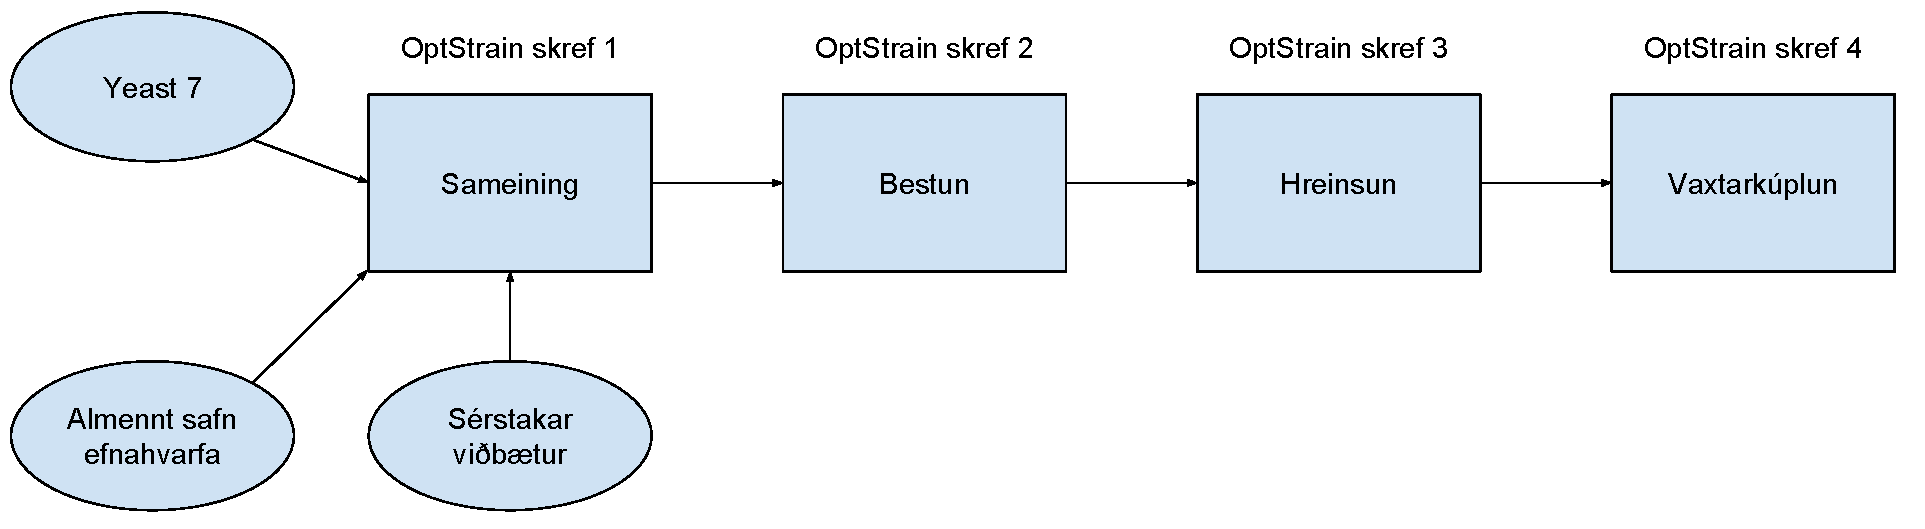
\includegraphics[width=\textwidth]{Pics/OptStrainOverview}
\end{figure}


\section{Inngangur}

Þó nokkur fordæmi eru fyrir því að erfðabreyta gersveppum til nota í matvælaiðnaði \cite{dequin2001potential}.

\section{Aðferð}
% Fyrsti textinn sem er skrifaður
% Byrja á undirtitlum
% Mikilvægt að strúktúra málsgreinarnar vel
% Mikilvægt að tengja 
\subsection{Framleiðsla í hefðbundnu gerjunarferli}
\subsubsection{Kolefnisgjafar og gefin skilyrði}
Gerjanlegu sykrurnar í virti eru frúktósi, glúkósi, súkrósi, maltósi og maltótríósi. Þar vega mest hlutverk maltósa, frúktósa og maltótríósa \cite{otter1967determination}. Maltótríósi er ekki til staðar í Yeast7 líkaninu og hlutverk annarra kolefnisgjafa er óverulegt, svo til einföldunar voru einungis maltósi og glúkósi. Valin hlutföll eru 1 hlutur glúkósa á móti 2 hlutum maltósa. Gerjun fer fram við loftfirrtar aðstæður, sem gert er ráð fyrir í líkaninu.
\subsection{OptStrain}
\label{sec:optstrain}
\subsubsection{Almenn lýsing}
\subsubsection{Útfærsla}

\section{Niðurstöður}

Mikilvæg efni eru: ethanol, isoamyl acetate (bananabragð), glycerol (sæta), urea (óbragð) \cite{dequin2001potential}.

% Undirtitlar hér líka

\section{Samantekt}
% Byrjar oftast eins: Here we set out to...

% \paragraph{Samantekt á niðurstöðum}
% \paragraph{Hvernig falla niðurstöðurnar að öðrum þekktum niðurstöðum}
% Ræða hvern undirtitil í niðurstöðu-hlutanum sérstaklega
% Aftur samantekt á síðustu málsgreinum, summary of impact

\appendix
%%%%%%%%%%%%%%
% HEIMILDASKRÁ
%%%%%%%%%%%%%%
\bibliographystyle{plain}
\bibliography{bioinfo.bib}

\end{document}